% \documentclass[a4paper,11pt]{article}
% \usepackage[hyperref]{beamerarticle}

\documentclass[final]{beamer}

\usepackage[hangul]{kotex}
\usepackage{amsfonts,amsmath,xob-amssymb}

\usepackage{amsthm}
\newtheorem{defn}{Definition}
\newtheorem{thm}{Theorem}

\usepackage{cancel}
\graphicspath{{./_img/06/}}

\usepackage{graphicx}
\usepackage{media9}
\usepackage{tikz}
\usepackage{textpos}
\usepackage{multirow}

\mode<presentation>{
	\usetheme{Madrid}
	\usecolortheme{default}
	\usefonttheme{professionalfonts}
}

\def\b{\boldsymbol}

\mode<article>{
\usepackage{fullpage}
}
\usepackage{ulem}

\newcommand{\bb}{\mathbb}
\newcommand{\bd}{\mathbf}
\newcommand{\p}{\partial}

\newcounter{saveenumi}
\newcommand{\seti}{\setcounter{saveenumi}{\value{enumi}}}
\newcommand{\conti}{\setcounter{enumi}{\value{saveenumi}}}

\newcommand{\mail}{\url{mailto:experiment.namun@gmail.com} }


\title{행동경제학 (1)}
\subtitle{행동경제학의 기원 및 기본 개념}
\author[조남운]{허준석$\rightarrow$이동한$\rightarrow$\emph{조남운}\\\mail}

\begin{document}
	
\begin{frame}[t]{}
	\maketitle
\end{frame}
%--- Next Frame ---%

\begin{frame}[t]{목차}
	\tableofcontents
\end{frame}
%--- Next Frame ---%

\section{Age of Behavioral Economics?} % (fold)
\label{sec:age_of_behavioral_economics}

\begin{frame}[t]{행동경제학의 대유행}
	\begin{columns}
		\column{.6\textwidth}
		\begin{itemize}
			\item 경제학 안팎의 현상
			\item 경제학 내부: 기존 체계에 대한 반성
			\item 경제학 외부: 
			\begin{itemize}
				\item 현실에 대한 설명력에 대한 필요성
				\item 정책적 효력에 대한 테스트의 필요성
			\end{itemize}
		\end{itemize}
		\column{.4\textwidth}
		\fbox{
\includegraphics[width=11em]{BE.jpg}}
	\end{columns}
\end{frame}
%--- Next Frame ---%

\begin{frame}[t]{우리는 행동경제학에서 무엇을 배울 것인가?}
	\begin{columns}
		\column{.6\textwidth}
		\begin{itemize}
			\item 심리학과 행동경제학
			\item 행동경제학은 보편적인 지침이 될 수 있을까?
			\item 행동경제학은 왜 경제학계에서 발언력을 획득하게 되었을까?
		\end{itemize}
		\column{.4\textwidth}
		\fbox{
\includegraphics[width=11em]{psychology.jpg}}
	\end{columns}
\end{frame}
%--- Next Frame ---%

\begin{frame}[t]{경제학 안과 밖에서의 행동경제학}
	\begin{columns}
		\column{.6\textwidth}
		\fbox{
\includegraphics[width=11em]{where.jpg}}
		\column{.4\textwidth}
		\begin{itemize}
			\item 행동경제학은 어떻게 경제학에 편입되었나?
			\item 행동경제학은 경제학의 어떤 측면을 보완해주는가?
			\item 행동경제학은 어디로 가고 있는가?
			\item 추천서적: 가격은 없다
		\end{itemize}
	\end{columns}
	
\end{frame}
%--- Next Frame ---%

% section age_of_behavioral_economics (end)

\section{Economics of Uncertainty} % (fold)
\label{sec:economics_of_uncertainty}

\begin{frame}[t]{St. Petersburg Paradox}
	\begin{columns}
		\column{.6\textwidth}
		\begin{itemize}
			\item 다음과 같은 단순한 도박 $G$가 있음
			\begin{enumerate}
				\item 동전을 던져서: (1) 앞면이 나오면 기회가 다시 주어짐. (2) 뒷면이 나오면 1달러를 주고 끝남
				\item 동전을 던져서: (1) 앞면이 나오면 또 던짐. (2) 뒷면이 나오면 2달러를 주고 끝남
				\item 동전을 던져서: (1) 앞면이 나오면 또 던짐. (2) 뒷면이 나오면 $2^2=4$ 달러를 주고 끝남
				\item ... 이런 식으로 앞면이 총 $k$번 나오면 $2^{k-1}$의 상금을 얻을 수 있음
			\end{enumerate}
			% \item 이 도박의 ``적정 가격''은 얼마인가? 
		\end{itemize}
		\column{.4\textwidth}
		{\includegraphics[width=11em]{daniel_Bernoulli.jpg}}
	\end{columns}
\end{frame}
%--- Next Frame ---%

\begin{frame}[t]{St. Petersburg Paradox (Calculation)}
	\begin{itemize}
	\item Expected value? 
	%
	\begin{align*}
	\hspace{-2em}\mathbb{E}(G)&= 1 \times \frac{1}{2} + 2 \times \frac{1}{4} + 4 \times \frac{1}{8} + \cdots + 2^{k-1} \times \frac{1}{2^{k-1} \times 2} + \ldots \\
	& = \frac{1}{2} + \frac{1}{2} + \ldots \\
	& = \infty
	\end{align*}
	%
	\item 그럼, 이 도박에 1억의 가격을 매기면 사람들이 할까? \\
	(1억 < $\infty$ ?)
	\item Daniel Bernoulli (1738) 
	\end{itemize}
\end{frame}
%--- Next Frame ---%

\begin{frame}[t]{Bernoulli's Solution}
	\begin{itemize}
	\item Not value, but utility!
	\item Money value to economic agent
	\item For example, $u(m)=\ln{m}$: 
	%
	\begin{align*}
	\hspace{-2em}\mathbb{E}(U(G))&= \ln{1} \times \frac{1}{2} + \ln{4} \times \frac{1}{8} + \cdots + \ln{2^{k-1}} \times \frac{1}{2^{k-1} \times 2} + \ldots \\
	& = 0.693147.
	\end{align*}
	%
	\item 실제의 효용은 보기보다 훨씬 낮을 수 있다! 
	\item John von Neumann {\&} Oskar Morgenstern의 일반화
	\end{itemize}
\end{frame}
%--- Next Frame ---%

\subsection{Paradox} % (fold)
\label{ssec:precursors}

\begin{frame}[t]{Allais Paradox (1)}
	%
	\begin{table} 
	\setlength{\tabcolsep}{1.2em}
	\begin{tabular}{|c|c||c|c|} \hline
	\multicolumn{2}{|c||}{GAMBLE 1A}&\multicolumn{2}{c|}{GAMBLE 1B} \\ \hline
	Winnings & Prob. & Winnings & Prob. \\ \hline
	\multirow{3}[2]{*}{1M} & \multirow{3}[2]{*}{1} & 1M & 0.89 \\ \cline{3-4}
	& & 0M & 0.01 \\  \cline{3-4}
	& & 2.5M & 0.10 \\  \hline
	\end{tabular}
	\caption{Allais 실험 1}\label{tab:01}
	\end{table}
	%
	\begin{itemize}
		\item 당신의 선택은? 
		\item 일단 결과를 기억해두고 실험 2로 넘어가보자. 
	\end{itemize}
	%
\end{frame}
%--- Next Frame ---%


\begin{frame}[t]{Allais Paradox (2)}
	%
	\begin{table}
	\setlength{\tabcolsep}{1.2em}
	\begin{tabular}{|c|c||c|c|} \hline
	\multicolumn{2}{|c||}{GAMBLE 2A}&\multicolumn{2}{c|}{GAMBLE 2B} \\ \hline
	Winnings & Prob. & Winnings & Prob. \\ \hline
	0M & 0.89 & \multirow{2}[2]{*}{0M} & \multirow{2}[2]{*}{0.9} \\ \cline{1-2}
	\multirow{2}[2]{*}{1M} & \multirow{2}[2]{*}{0.11} & & \\  \cline{3-4}
	& & 2.5M & 0.10 \\ \hline
	\end{tabular}
	\caption{Allais 실험 2}\label{tab:02}
	\end{table}
	%
	\begin{itemize}
		\item 당신의 선택은?
		\item 어떤 선택을 한 사람들은 ``합리적''이지 않을까?
	\end{itemize}
	%
\end{frame}
%--- Next Frame ---%

\begin{frame}[t]{합리성에 기반한 검토: 1A, 2B를 선택한 경우에 대해서}
	\begin{itemize}
		\item 실험 (1)의 경우: 1A를 선호했다면..
		{\small 
		\begin{align*}
		1.00 \times U(1M) > 0.89 \times U(1M) + 0.01 \times U(0M)  + 0.10 \times U(2.5M) 
		\end{align*}
		}
		\item 실험 (2)의 경우: 2B를 선호했다면.. 
		{\small 
		\begin{align*}
		\mathbf{0.89 \times U(0M)} + 0.11 \times U(1M) & < \mathbf{0.90 \times U(0M)}  + 0.10 \times U(2.5M) \\
		\color{red}{0.11 \times U(1M)}  & < \mathbf{0.01 \times U(0M)} + 0.10 \times U(2.5M) \\
		\color{red}{1.00 \times U(1M) - 0.89 \times U(1M)} & < 0.01 \times U(0M) + 0.10 \times U(2.5M) 
		\end{align*}
		}
		\item 따라서, 1A, 2B 각각 선택한 사람을 모두 설명할 수 있는 하나의 $U(x\$)$는 존재할 수 없다!
		{\small
		\begin{align*}
		1.00 \times U(1M) &< 0.89 \times U(1M) + 0.01 \times U(0M) + 0.1 \times U(2.5M) 
		\end{align*}
		}
	\end{itemize}
\end{frame}
%--- Next Frame ---%

\begin{frame}[t]{Maurice Allais}
	\begin{columns}[c]
	\column{18em}
	\begin{itemize}
		\item 불확실성 하의 선택에 대한 독자적인 접근 
		% \item 뽑을 수 없는 ``엑스칼리버'' 같은 패러독스? %무슨 얘기인지 모르겠음. 
		\item 불확실성 하에서 선택에 대해서는 어떻게 접근해야 할까? 
	\end{itemize}
	\column{12em}
	%\hspace{-1em}
	\fbox{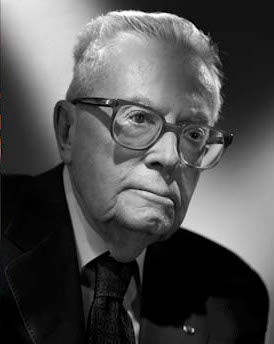
\includegraphics[width=11em]{MauriceAllais.jpg}}
	\end{columns}
\end{frame}
%--- Next Frame ---%

\begin{frame}[t]{Ellsberg Paradox}
	\begin{itemize}
	\item 30개의 빨간 공 그리고 60개의 검은 공 혹은 노란 공이 든 단지
	\end{itemize}
	%
	\vspace{1em}
	\begin{columns}[c]
	\column{11em}
	Gamble 1 is \\[1em]
	$
	\begin{cases}
	\text{1M}& \text{if ball is red (1A)} \\
	\text{1M}& \text{if ball is black (1B)}
	\end{cases}
	$
	\column{15em}
	Gamble 2 is \\[1em]
	$
	\begin{cases}
	\text{1M}& \text{if ball is red or yellow (2A)} \\
	\text{1M}& \text{if ball is black or yellow (2B)}
	\end{cases}
	$
	\end{columns}
	\vspace{1.5em}
	%
	\begin{itemize}
	\item 각각의 gamble에서 당신의 선택은? 
	\end{itemize}
\end{frame}
%--- Next Frame ---%

\begin{frame}[t]{Ellsberg Paradox (2)}
	\begin{itemize}
		\item If 1B 대신 1A를 선택했다면,
	\begin{align*}
	p_r{\,}U(1M) + (1-p_r) U(0M) & > p_b{\,}U(1M) + (1-p_b) U(0M)\\
	(p_r-p_b) \left( U(1M)-U(0M) \right) &>0.
	\end{align*}
	%
		\item If 2A 대신 2B를 선택했다면, (red or yellow = not black, black or yello = not red)
	%
	\begin{align*}
	(1-p_b)U(1M) + p_b{\,}U(0M)  & < (1-p_r)U(1M) + p_r{\,}U(0M)\\
	(p_b-p_r) \left( U(1M)-U(0M) \right) & >0.
	\end{align*}
	%
	\item 역시 동시 성립 불가능! 일관되지 않은 선택?
	\end{itemize}
\end{frame}
%--- Next Frame ---%

% subsection precursors (end)

\begin{frame}[t]{Misunderstanding on Economic Rationality}
	\begin{columns}[c]
	\column{18em}
	\begin{enumerate}
		\item 경제학에 따르면, 인간은 철저하게 계산하는 존재이고 이에 따라서 자신의 행동을 결정
		\item 현실에서 인간은 결코 이렇게 정확하게 계산할 수 없고 하지도 않음
		\item 따라서 경제학은 그 전제부터 잘못되었다고 보는 관점
	\end{enumerate}
	\column{12em}
	\fbox{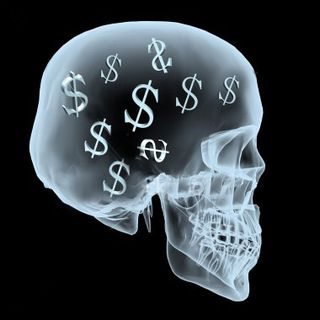
\includegraphics[width=11em]{rationality.jpg}}
	\end{columns}
\end{frame}
%--- Next Frame ---%

\begin{frame}[t]{Misunderstanding on Economic Rationality (2)}
	\begin{itemize}
		\item 경제학적 분석은 ``as if'' 
		\item 주어진 대안에서 뭔가를 선택하고, 그 선택이 ``일관성''을 지닌다면 
		\item 뭔가를 고른다는 것과 수학적인 분석은 완전히 일치!
		\item 일관성이란?\\[1em]
		\fbox{
		\begin{minipage}[c]{26em}
		$x$, $y$가 모두 $A$, $B$라는 선택 가능한 것들의 집합에 속해 있을 때 $A$만을 두고 $y$ 대신 $x$를 택했다면, $B$만을 두고 택할 때 $y$를 택해서는 안된다.
		\end{minipage}
		}
	\end{itemize}
\end{frame}
%--- Next Frame ---%

\begin{frame}[t]{Milton Friedman}
	\begin{columns}[c]
	\column{12em}
	\hspace{2em}
	\fbox{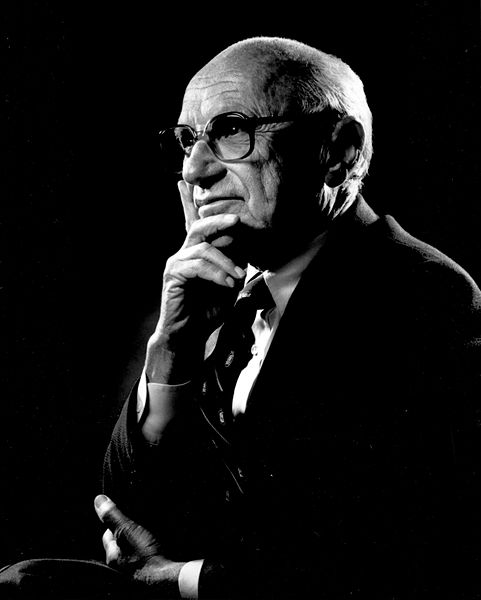
\includegraphics[width=11em]{Friedman.jpg}}
	\column{20em}
	\begin{quote}
	An expert billiard player makes shots as if they ``knew the complicated mathematical 
	formulas that would give the optimum directions of travel…could make 
	lightening calculations from the formulas,'' and could do what the formulas 
	require. (Friedman 1953)
	\end{quote}
	\end{columns}
\end{frame}
%--- Next Frame ---%

\begin{frame}[t]{Expected Utility Hypothesis}
	\begin{itemize}
		\item 불확실성 하에서 어떻게 합리적인 효용을 구축할 것인가?  
		\item von Neumann {\&} Morgenstern: 
		\\~~~몇가지 공리(axioms)를 가정하면 EU가 합리적인 효용을 대변
		\item 불확실성을 지닌 대안 G가 $n$가 가능성을 지닐 때 이 대안의 효용은 
		%
		\begin{align*}
		EU(G)=p_1 U(x_1) + p_2 U(x_2) + \cdots + p_n U(x_n) . 
		\end{align*}
	\end{itemize}
\end{frame}
%--- Next Frame ---%

\begin{frame}[t]{Expected Utility Hypothesis (2)}
	\begin{center}
	\fbox{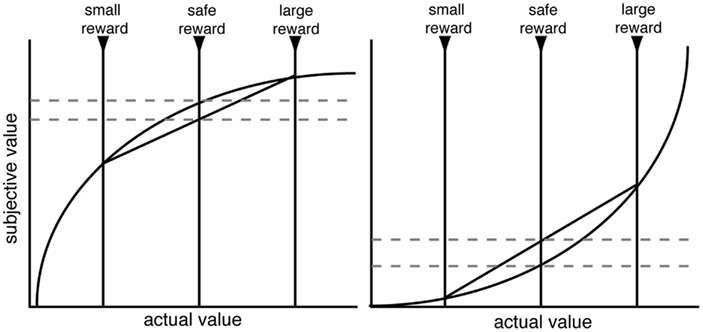
\includegraphics[width=19em]{risk.jpg}}
	\end{center}
	\begin{itemize}
		\item risk를 측정할 수 있게 되었다. 
		\item $U(\cdot)$을 어떻게 놓는냐에 따라서 risk에 대한 태도를 구분 
		\begin{enumerate}
			\item risk-averse (위험 기피)
			\item risk-neutral (위험 중립) 
			\item risk-taking (위험 감수)
		\end{enumerate}
	\end{itemize}
\end{frame}
%--- Next Frame ---%

\begin{frame}\frametitle{Expected Utility Hypothesis (con't)}\vspace{3.5em}
\begin{itemize}
\item 무척 훌륭한 정식화였지만, 잃은 것은 
	\begin{enumerate}
		\item Ordinality vs. Cardinality 
		\item 불확실성은 cardinality로 충분히 표현되지 않는다. 
	\end{enumerate}
\item 앞서 경제학의 엄밀한 분석은 ordinality를 통해 확보. \\ 그런데, risk가 연관되면서 다시 cardinality를 불러들임. 
\item 불확실성 하에서 판단은 일관된 cardinality를 갖는가?  
\end{itemize}
\end{frame}
%
\begin{frame}\frametitle{Back to Allais}\vspace{3em}
%\begin{columns}[c]
%\column{18em}
\begin{itemize}
	\item 원래 Savage에게 던졌던 낚시 질문은 다음의 세가지 
	\begin{enumerate}
	\item  $1 \times$ 1M~~~{\color{red}{vs.}}~~~ $0.89 \times$ 1M + $0.10 \times$ 2.5M + $0.01 \times$ 0M 
	\item  $0.11 \times$ 1M + $0.89 \times$ 0M~~~{\color{red}{vs.}}~~~$0.10 \times$ 2.5M + $0.89 \times$ 0M
	\item  $0.89 \times x$ + $0.11 \times$ 1M~~~{\color{red}{vs.}}~~~
	$0.89 \times x$ + $0.10 \times$ 2.5M + $0.01 \times$ 0	M
	\end{enumerate}
	\item 2와 3은 같은 질문인가?
	\item 독립성(independence) 가정에 따르면 그러하다. \\그렇다면, 만일 $x$가 1M이라면?   
\end{itemize}
%\column{12em}
%\fbox{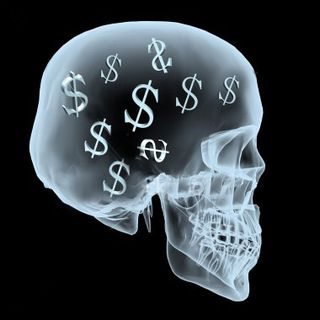
\includegraphics[width=11em]{rationality.jpg}}
%\end{columns}
\end{frame}
%
\begin{frame}\frametitle{Remixed by Richard Zechkhauser}\vspace{2em}
\begin{columns}[c]
\column{18em}
\begin{itemize}
	\item Russian Roulette with six cartridges
\fbox{\parbox{.80\textwidth}{
	\begin{enumerate}
		\item 총알이 딱 하나 들어 있습니다. \\하나 사시겠습니까?
		\item 총알이 4개 들어 있습니다. \\하나 사시겠습니까? 
	\end{enumerate}
}}
%
\fbox{\parbox{.8\textwidth}{\begin{enumerate}
		\item 총알이 꽉 차 있습니다. \\하나 사시겠습니까? 
		\item 총알이 4개 들어 있습니다. \\하나 사시겠습니까?
	\end{enumerate}}}
\end{itemize}
\column{14em}
\fbox{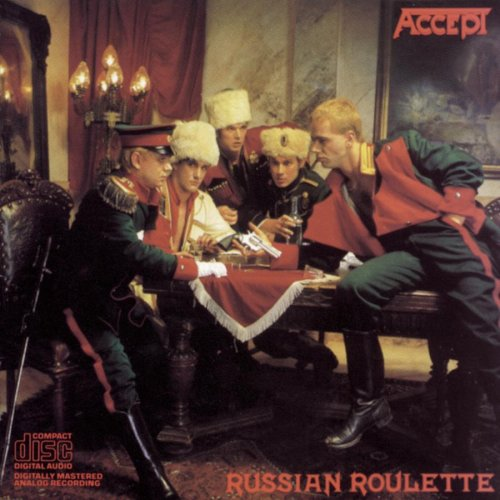
\includegraphics[width=13em]{album-russian-roulette.jpg}}
\end{columns}
\end{frame}
%
\section{Here Comes Behavioral Economics!}
%
\begin{frame}\frametitle{Connecting Psychology to Economics}\vspace{3em}
\begin{columns}[c]
%
\column{18em}
\begin{itemize}
	\item 경제학에서 간헐적으로 제기된 anomalies 
	\item 심리학은 경제적 선택에 상대적으로 무관심 
	\item 이 두개의 틈을 파고 든 학자들이\\
	Daniel Kahneman and Amos Tversky
	\item Prospect theory
\end{itemize}
%
\column{12em}
\fbox{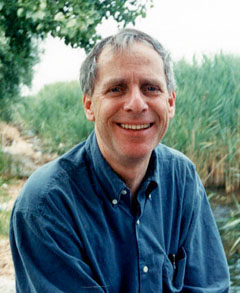
\includegraphics[width=11em]{tversky.jpg}}
Tversky
\end{columns}
\end{frame}
%
\begin{frame}\frametitle{Prospect Theory}\vspace{1.5em}
%
\begin{itemize}
\item 다음과 같은 멋진 선물을 제공한다면,
\begin{table} 
\setlength{\tabcolsep}{1.2em}
\begin{tabular}{|c|c||c|c|} \hline
\multicolumn{2}{|c||}{GAMBLE 1A}&\multicolumn{2}{c|}{GAMBLE 1B} \\ \hline
Winnings & Prob. & Winnings & Prob. \\ \hline
\multirow{2}[2]{*}{1M} & \multirow{2}[2]{*}{1} & 2M & 0.5 \\ \cline{3-4}
& & 0M & 0.5 \\  \hline
\end{tabular}
\caption{K-T 실험 1}\label{tab:03}
\end{table}
%
\item 당신의 선택은? 
\item 일단 선택을 기억해두기로 하고. 
\end{itemize}
%
\end{frame}
%
\begin{frame}\frametitle{Prospect Theory (con't)}\vspace{1.5em}
%
\begin{itemize}
\item 일단 당신에게 2M을 선물한 뒤, 
\begin{table} 
\setlength{\tabcolsep}{1.2em}
\begin{tabular}{|c|c||c|c|} \hline
\multicolumn{2}{|c||}{GAMBLE 2A}&\multicolumn{2}{c|}{GAMBLE 2B} \\ \hline
Winnings & Prob. & Winnings & Prob. \\ \hline
\multirow{2}[2]{*}{$-1$M} & \multirow{2}[2]{*}{1} & $0$M & 0.5 \\ \cline{3-4}
& & $-2$M & 0.5 \\  \hline
\end{tabular}
\caption{K-T 실험 2}\label{tab:04}
\end{table}
%
\item 당신의 선택은? 
\item 이것은 일관된 것일까? 
\end{itemize}
%
\end{frame}
%
\begin{frame}\frametitle{Prospect Theory (con't)}\vspace{1.5em}
%
\begin{itemize}
\item ``K-T 실험 1''에서 만일 1A를 택했다면, 
%
\begin{align*}
1 \cdot U(1M) > 0.5 \cdot U(2M) + 0.5 \cdot U(0M)
\end{align*}
%
\item ``K-T 실험 2''에서 만일 2B를 택했다면, 
%
\begin{align*}
1 \cdot U(2M-1M) < 0.5 \cdot U(2M) + 0.5 \cdot U(2M-2M)
\end{align*}
%
\item 무엇이 이런 ``역설''을 만들어내었는가? 
\end{itemize}
%
\end{frame}
%
\begin{frame}\frametitle{Reference Point \& Loss Aversion}\vspace{1.5em}
%
\begin{columns}[c]
\column{18em}
\begin{itemize}
\item 심리적으로 준거점에 닻을 내리게 되면, 이는 경제적 판단에 기준이 된다. 
\item 이 준거점을 기준으로, 
$(+)$에 대해서는 위험 회피를, $(-)$에 대해서는 위험 감수 선택 
\item $(-)$의 위험 감수를 ``손실 회피''라고 부른다.  
\item 예를 들어, 왜 도박에 빠져들게 되는가? 
\end{itemize}
%
\column{12em}
\fbox{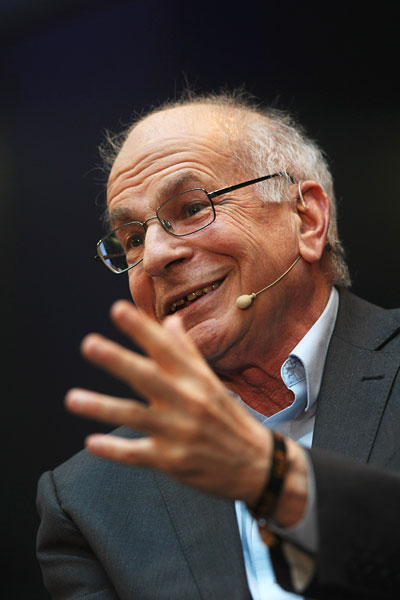
\includegraphics[width=11em]{kahneman.jpg}}
Kahneman
\end{columns}
\end{frame}
%
\begin{frame}\frametitle{Reference Point \& Loss Aversion (con't)}\vspace{3em}
%
\begin{columns}[c]
\column{15em}
\begin{itemize}
\item wealth가 $(+)$인 영역에 대해서는 위험 회피 
\item wealth가 $(-)$인 영역에 대해서는 손실 회피 
\item 결국 reference point에 따라서 경제적 행동이 극적으로 변한다. 
\end{itemize}
%
\column{14em}
\hspace{-1em}
\fbox{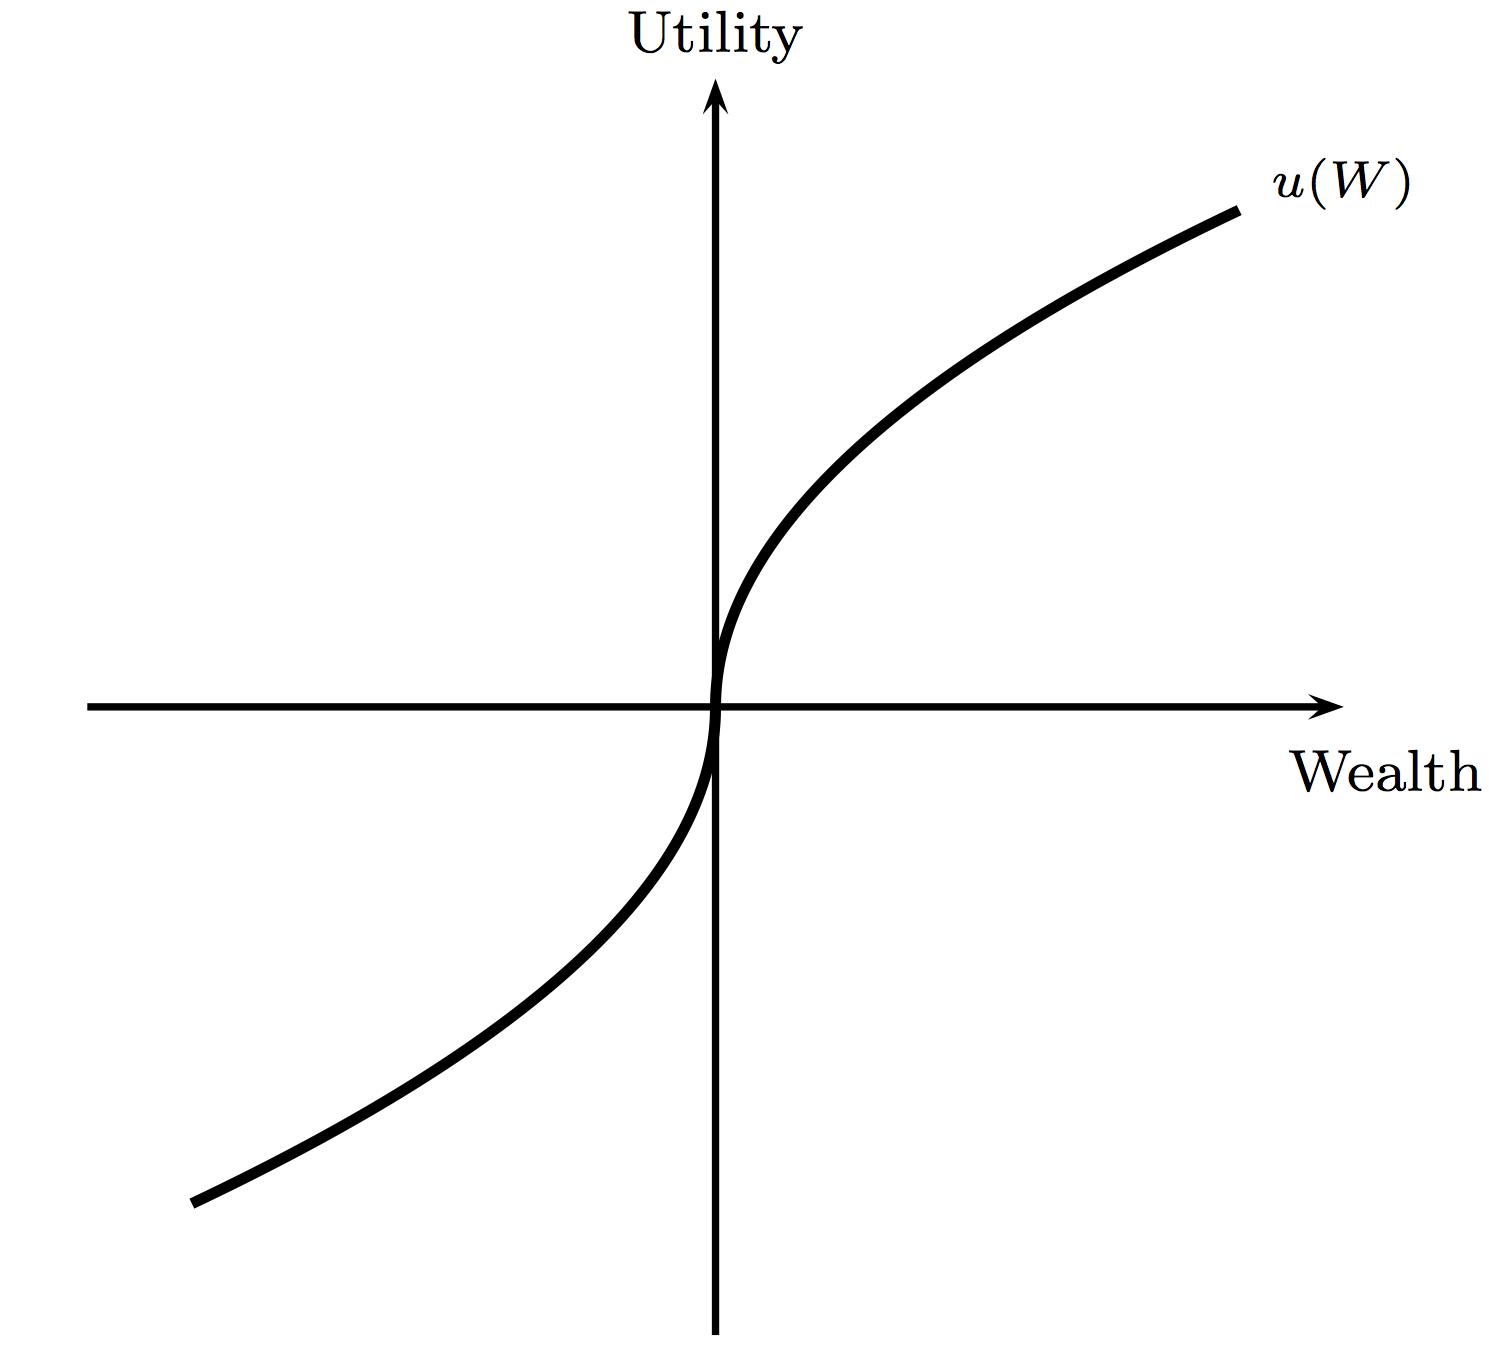
\includegraphics[width=14em]{lossaversion.png}}
\end{columns}
\end{frame}
%
\section{Some Key Concepts and Cases}
%
\begin{frame}\frametitle{Anchoring}\vspace{3em}
%
\begin{columns}[c]
\column{18em}
\begin{itemize}
\item 카너만과 트버스키의 UN국가 실험 
\item 전혀 관계없는 정보가 판단에 영향을 준다.
\item 새끼거위의 법칙 혹은 각인 효과(imprinting effect)
\item 톰 소여의 펜스 칠하기 %Perl King의 흑진주 도입 %무슨 얘기일까?
\end{itemize}
\column{12em}
\hspace{-1em}
\fbox{
\includegraphics[width=12em]{tom.jpg}}
\end{columns}
\end{frame}
%
\begin{frame}\frametitle{Endowment Effect}\vspace{3em}
%
\begin{columns}[c]
\column{12em}
\vspace{-2em}
\begin{align*}
WTA > WTP 
\end{align*}
\vspace{-1em}
%
\begin{itemize}
\item Willingness to Accept\\ Willingness to Pay 
\item Thaler의 실험
\item 이케아 효과 
\end{itemize}
\column{18em}
\hspace{-1em}
\fbox{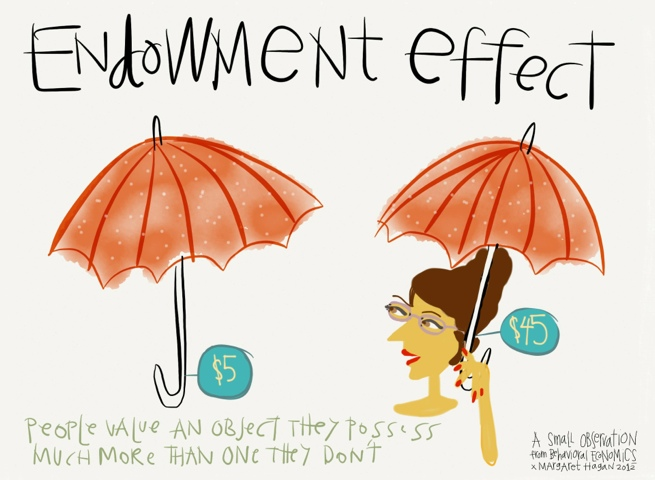
\includegraphics[width=18em]{endowment.jpg}}
\end{columns}
\end{frame}

\begin{frame}[t]{유보가격에 대한 행동실험}
	\begin{itemize}
		\item 도박1: 
		\begin{itemize}
			\item 80\% - 50,000원
			\item 20\% - 0원
		\end{itemize}
		\item 도박2:
		\begin{itemize}
			\item 10\% - 400,000원
			\item 90\% - 0원
		\end{itemize}
		\item 응답: \url{https://goo.gl/forms/IujoU0nZtRi4pgC32}
		\item ​응답 결과에 의거하여 가상 시장을 만들고 임의의 순서로 조건에 맞는 사람들이 거래를 하며, 최종 보유하고 있는 도박은 실제 컴퓨터로 도박을 개별실시하여 그 결과액을 거래중 보유하게 된 돈과 합산할 것임. 운에 의한 효과를 완화하고자 거래 순서를 랜덤하게 섞어 100회 반복한 뒤 총합금액을 최종 보상으로 산정할 것임. 
	\end{itemize}
\end{frame}
%--- Next Frame ---%

%
\begin{frame}\frametitle{Preference Reversal}\vspace{3em}
%
\begin{columns}[c]
\column{12em}
\begin{itemize}
\item 복권의 가치는 가장 높은 당첨금이 결정하면서도, 
\item 당첨확률이 높은 복권을 좋아한다. 
\item 선택은 그것이 제시되는 맥락 혹은 틀에 의존한다. 
\end{itemize}
\column{18em}
600명의 사람이 있을 때 \\[1em]
\fbox{
\begin{minipage}[c]{17em}
\begin{enumerate}[a)]
\item 200명을 확실히 구할 수 있다. 
\item $^1/_3$의 확률로 600명을 구하거나,\\ $^2/_3$의 확률로 다 죽는다.  
\end{enumerate}
\vspace{-0.5em}
\end{minipage}
}
\\[1em]
\fbox{
\begin{minipage}[c]{17em}
\begin{enumerate}[A)]
\item 400명이 확실히 죽게 된다. 
\item $^1/_3$의 확률로 모두 살게 되거나,\\ $^2/_3$의 확률로 다 죽는다.  
\end{enumerate}
\vspace{-0.5em}
\end{minipage}
}
\end{columns}
\end{frame}
%

\begin{frame}\frametitle{Preference Reversal (con't)}\vspace{1em}
%
일단 두 사람(A,B)을 뽑아 봅시다. \\[1em]
\fbox{
\begin{minipage}[c]{30em}
\begin{enumerate}[I)]
\item A에게 200만원을 빼았는다.
\item B에게 300만원을 준다. 
\end{enumerate}
\vspace{-0.5em}
\end{minipage}
}
\\[3em]
\fbox{
\begin{minipage}[c]{14em}
\begin{enumerate}[A)]
\item A는 게을러서 \\ 200만원 손해 
\item B는 부지런히 \\ 일해서 300만원 이득 
\end{enumerate}
\vspace{-0.5em}
\end{minipage}
}~~~~
\fbox{
\begin{minipage}[c]{14em}
\begin{enumerate}[A)]
\item A는 한국에서 공장을 운영해서 \\ 200만원 손해 
\item B는 중국으로 공장을 옮겨서 \\ 300만원 이득 
\end{enumerate}
\vspace{-0.5em}
\end{minipage}
}
\end{frame}
%
\begin{frame}\frametitle{Hyperbolic Discounting}\vspace{3.5em}
\begin{columns}
\column{14em}
\begin{itemize}
	\item 헬스클럽의 장기할인 전략
	\item 현재 시점에서 보는 미래, \\ 그리고 현재가 된 미래  
	\item ``Present bias''
	\item 왜 벼락치기인가? \\ 왜 알람을 끄는가?
\end{itemize}
\column{16em}
\fbox{
\includegraphics[width=16em]{health.jpg}}
\end{columns}
\end{frame}
%
\begin{frame}\frametitle{Hyperbolic Discounting (con't)}\vspace{-1em}
\begin{center}
Exponential vs Hyperbolic\\[1em]
\end{center}
\hspace{-1em}\fbox{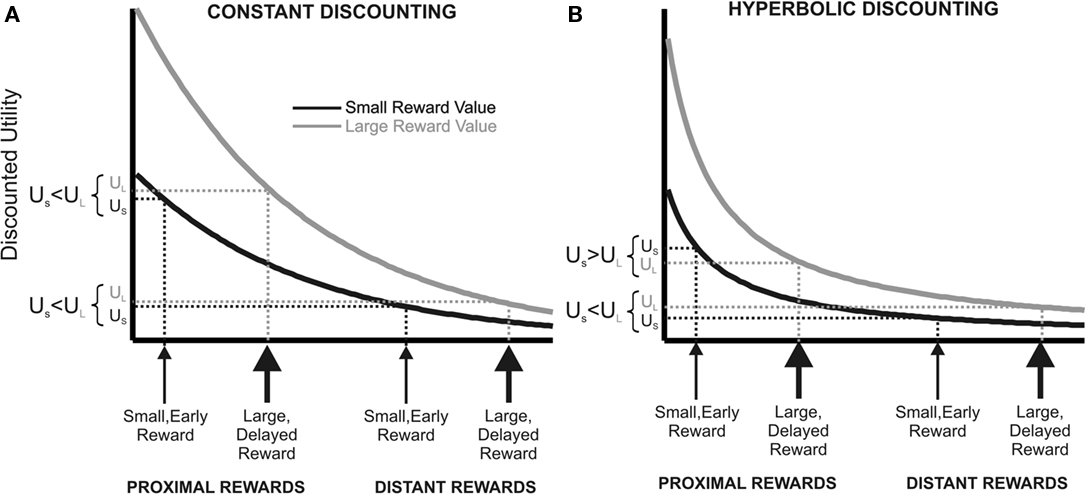
\includegraphics[height=.7\textheight]{exvshy.jpg}}
\end{frame}
%

\section{Rationality in Action}
%
\begin{frame}\frametitle{Sherlock Holmes}\vspace{3.5em}
%
\begin{columns}[c]
\column{14em}
\hspace{2em}
\fbox{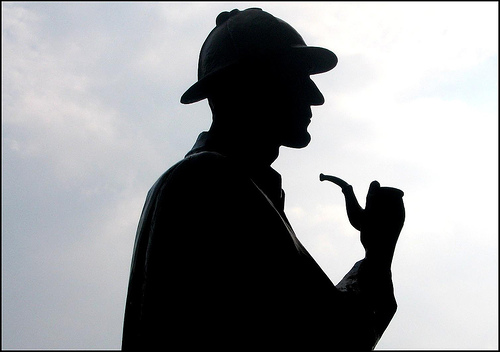
\includegraphics[width=14em]{sherlock-holmes1.jpg}}
\column{16em}
\begin{quote}
``In solving a problem of this sort, the grand thing is to be able to reason backwards. That is a very useful accomplishment, and a very easy one, but people do not practise it much.''
\end{quote}
\end{columns}
\end{frame}
%
\begin{frame}\frametitle{Ultimatum Games}\vspace{3.5em}
%
\begin{columns}[c]
\column{16em}
\begin{itemize}
\item 실제로 한번 해보자. 
\item What's the motive
\item More and More
\begin{enumerate}
	\item Dictator game 
	\item Ian Stewart's Pirate game 
\end{enumerate}
\end{itemize}
\column{14em}
\hspace{-2em}
\fbox{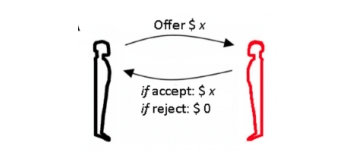
\includegraphics[width=14em]{ug.png}}
\end{columns}
\end{frame}
%
\begin{frame}\frametitle{Inequality Aversion}\vspace{-1em}
\begin{align*}
U_i(x)=\overbrace{x_i}^{(a)} - \alpha_i \overbrace{\max\{x_j-x_i,0\}}^{(b)}-\beta_i \overbrace{\max\{x_i-x_j,0\}}^{(c)}
\end{align*}
%
\vspace{-1em}
\begin{enumerate}[(a)]
	\item 원래 배분이 주는 물질적 가치 
	\item 남이 나보다 더 가져가서 생기는 비효용 
	\item 내가 남보다 더 가져가서 생기는 비효용 
\end{enumerate}
\begin{itemize}
\item 만일 모든 사람이 이런 성향을 가지고 있지 않더라도, 일부가 그렇다면?
\item Homo economicus는 어떻게 행동하게 될까? 
\end{itemize}
\end{frame}
%
\section{Comments}
%
\begin{frame}\frametitle{Context Matters!}\vspace{3.5em}
\begin{columns}[c]
\column{15em}
\begin{itemize}
	\item BE(Behavioral Economics)의 가장 큰 교훈은 경제적인 행위가 맥락에 의존한다는 것  
	\item 인간들이 전체적으로 이성적인 결정을 내릴 수 있지만, 
	\item 보다 미시적인 맥락에서 판단은 맥락과 상황에 휘둘리게 된다. 
	\item Homo economicus vs Home $x$?
\end{itemize}
\column{16em}
\fbox{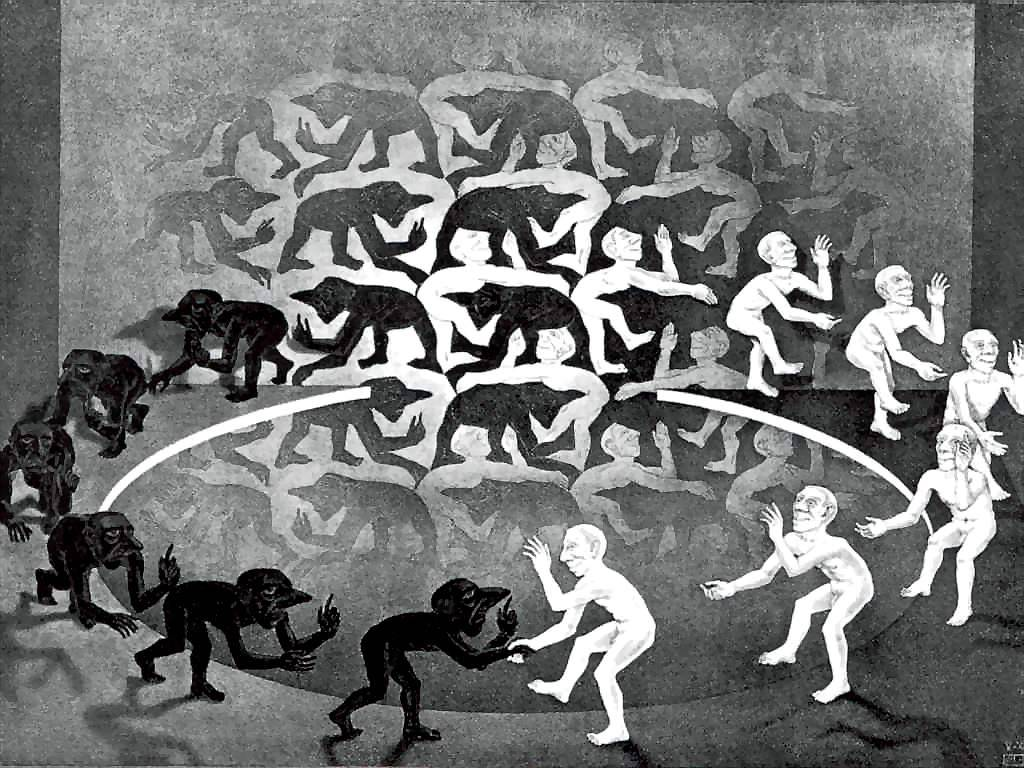
\includegraphics[width=16em]{escher_csg026_encounter.jpg}}
\end{columns}
\end{frame}
%
\begin{frame}\frametitle{Confirmation Bias}\vspace{.5em}
\begin{columns}[c]
\column{16em}
\begin{itemize}
	\item BE는 언제나 실험을 동반   
	\item 실험 조건의 미세한 변화에도 영향을 받을 수 있다. 
	\item BE는 방향일 뿐 결코 `결론'이 아니다! 
	\item Ultimatum game across cultures 
	\item 우리의 뇌는 매우 복합적인 진화의 산물
	\item 경제적 의사결정에 대한 연구라는 점을 염두 
\end{itemize}
\column{14em}
\hspace{0em}
\fbox{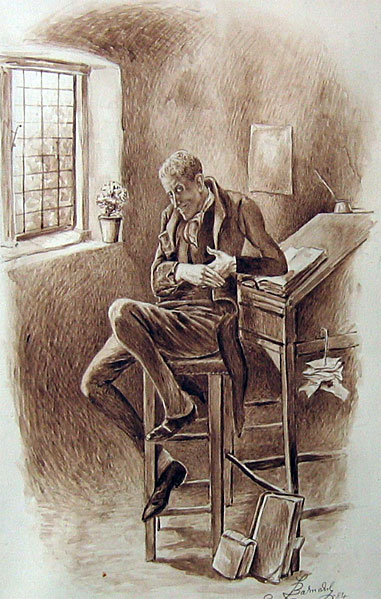
\includegraphics[width=12em]{Fred_Barnard07.jpg}}
\end{columns}
\end{frame}
%
\begin{frame}\frametitle{Imperfection to Be Cured? or Just Curse?}\vspace{2em}
\begin{columns}[c]
\column{18em}
\begin{itemize}
	\item BE의 결과들은 교정되어야 하는 불완전성인가? 아니면 인간의 한계인가?   
	\item 만일 교정에 성공했다면 지금쯤 모두가 Homo Economicus가 되었을 것!
	\item 많은 실험 결과들은 이러한 교정이 성공적이지 않다고 말해준다. 
	\item 때로는 이러한 잔재물 자체가 인간사에 유리하게 작용 
\end{itemize}
\column{12em}
\hspace{-1em}
\fbox{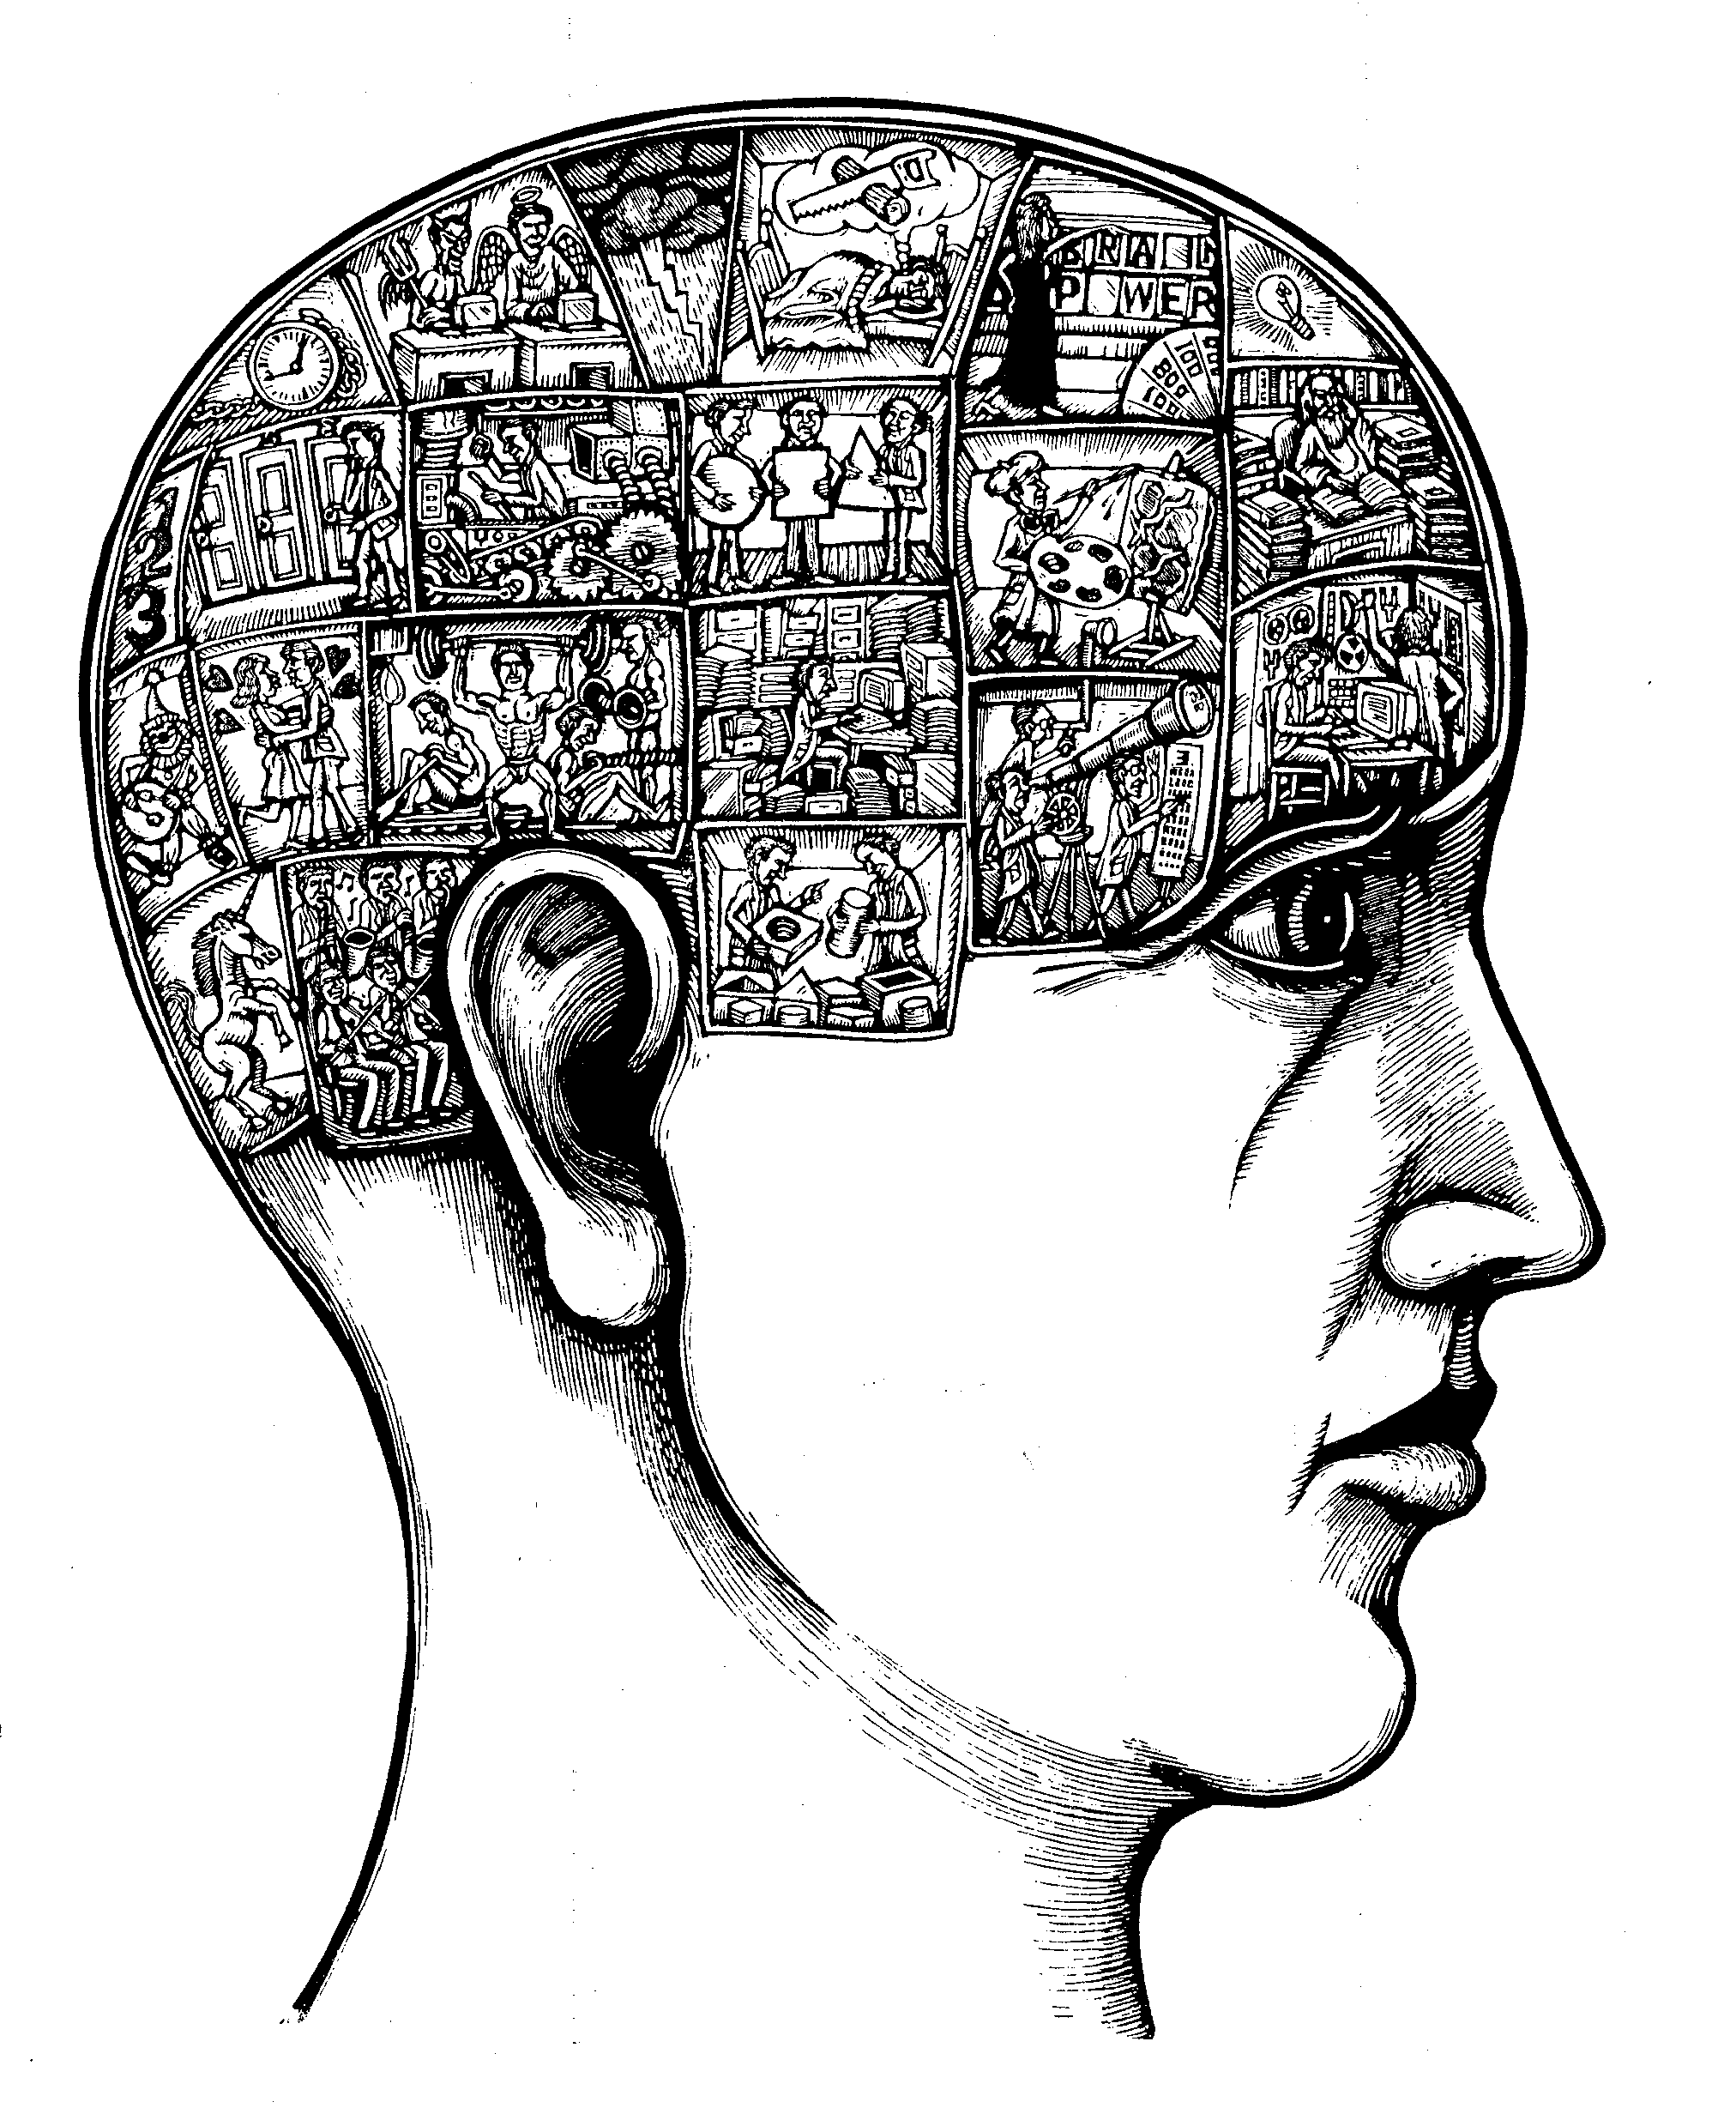
\includegraphics[width=12em]{phrenology-uiuc.png}}
\end{columns}
%
\end{frame}
%
\begin{frame}\frametitle{BE Is Not Panecea!}\vspace{3.5em}
\begin{columns}[c]
\column{17em}
\begin{itemize}
	\item Nudge: 인센티브를 훼손하지 않고 의사결정에 영향을 미치는 기법
	\item ``Nudge''는 때로는 효과적이다. 하지만 만병통치약?
	% \item 영국의 nudge unit은 보수당 정부의 잔꾀에 불과하다는 견해도 있음. 
	\item BE적 처방의 난무로 실제의 필요한 해결책이 지연되는 것은 아닐까?\\
\end{itemize}
\column{13em}
\hspace{0em}
\fbox{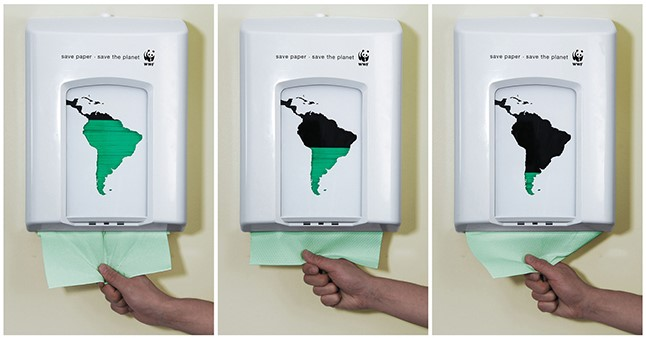
\includegraphics[width=12em]{nudge.jpg}}
\end{columns}
\end{frame}
%
\begin{frame}\frametitle{Complement, Not Substitute}\vspace{1.5em}
\begin{columns}[c]
\column{12em}
\hspace{0em}
\fbox{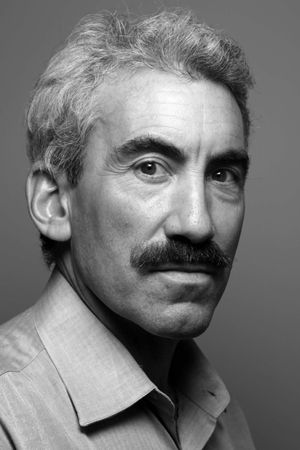
\includegraphics[width=11em]{loewenstein.jpg}}
\column{19em}
\begin{itemize}
\item George Loewenstein: \href{http://www.nytimes.com/2010/07/15/opinion/15loewenstein.html}{CLICK!}
\end{itemize}
\begin{quote}\small
``Behavioral economics should complement, not substitute for, more substantive economic interventions. If traditional economics suggests that we should have a larger price difference between sugar-free and sugared drinks, behavioral economics could suggest whether consumers would respond better to a subsidy on unsweetened drinks or a tax on sugary drinks.''
\end{quote}
\end{columns}
\end{frame}
%
\begin{frame}\frametitle{Gerd Gigerenzer}\vspace{2em}
\begin{columns}[c]
\column{17em}
\begin{itemize}
	\item 의사들에게 질문을 던져 봄. 
	\begin{enumerate}
		\item 여성들의 유방암 발병확률은 $1${\%}
		\item 유방암이 있을 경우 검사에 양성반응을 보일 확률은 $90${\%}
		\item 유방암에 없을 경우 검사에 양성반응을 보일 확률은 $9${\%}
	\end{enumerate}
	\item 어떤 여성이 검사에서 양성반응을 보였을 때 실제로 유방암에 걸렸을 확률은? 
\end{itemize}
\column{13em}
\hspace{0em}
\fbox{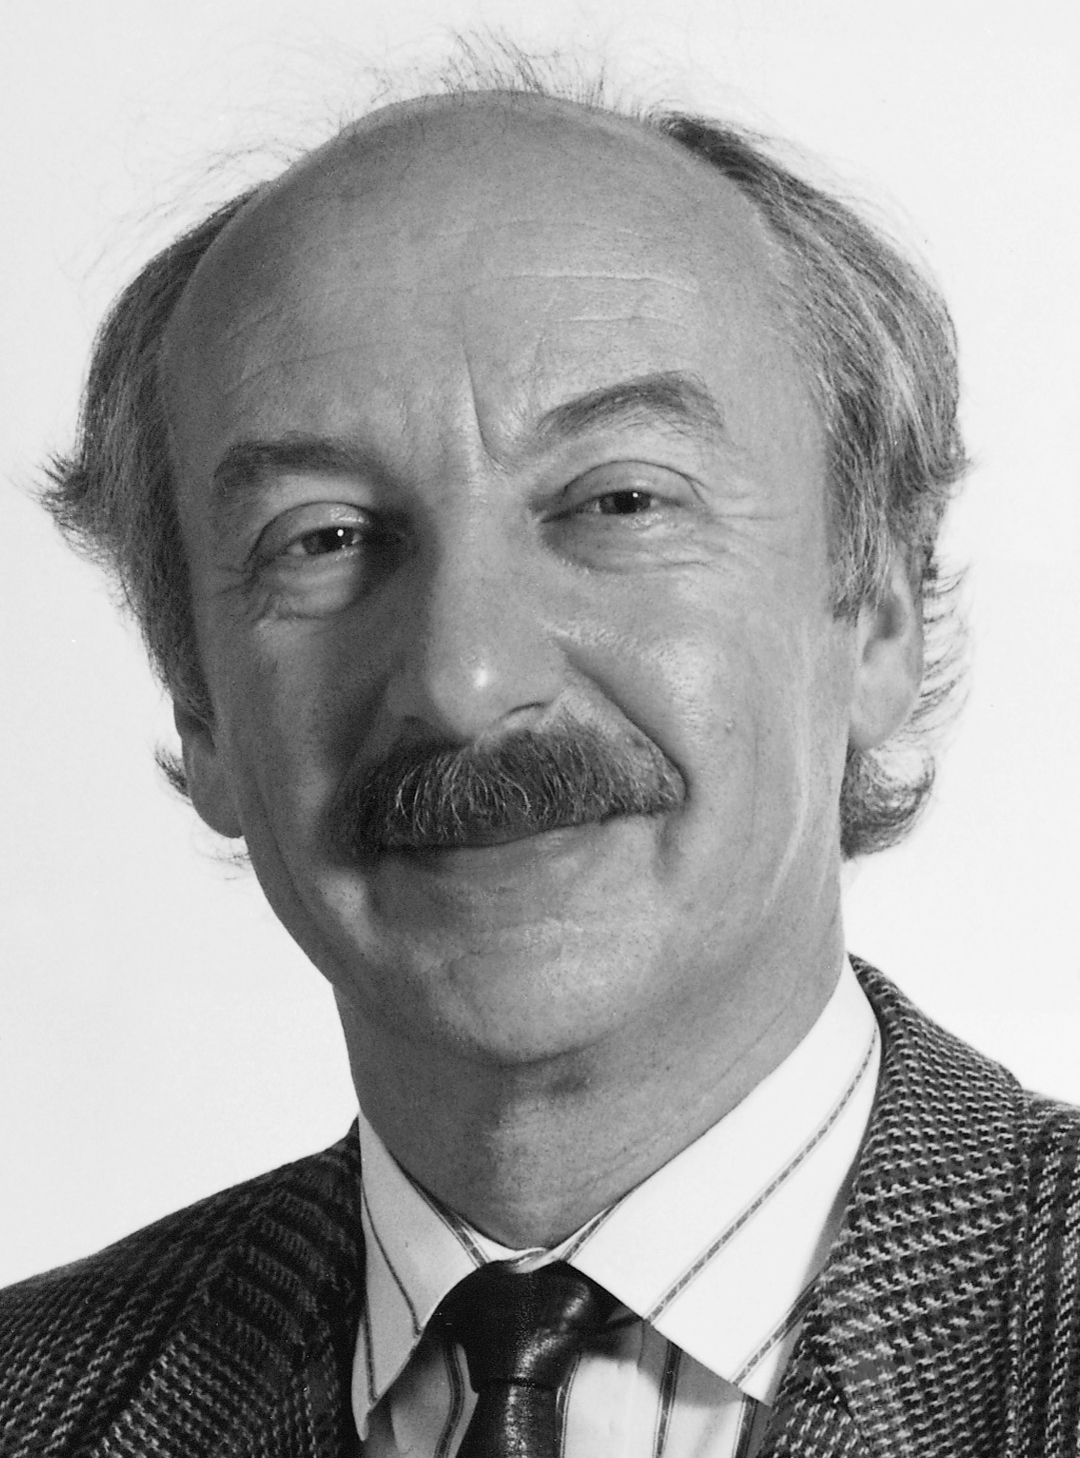
\includegraphics[width=12em]{Gigerenzer_300.jpg}}
\end{columns}
\end{frame}
%
\begin{frame}\frametitle{Gerd Gigerenzer (con't)}\vspace{1.5em}
\begin{columns}[c]
\column{13em}
\begin{itemize}
	\item 기본적으로 Bayes' Rule
	\item 확률이 아닌 빈도에 입각한 사고의 틀 
    \item 내가 아는 아주 휼륭한 `지식' 인터페이스!
    \item S. Strogatz의 해설 (\href{http://opinionator.blogs.nytimes.com/2010/04/25/chances-are/}{CLICK})
\end{itemize}
\column{17em}
\hspace{-0.5em}
\fbox{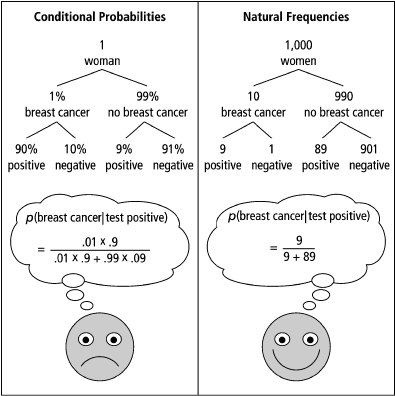
\includegraphics[width=17em]{gigerenzer_image_7.jpg}}
\end{columns}
\end{frame}

% section economics_of_uncertainty (end)

\end{document}